\section{Teori}
    I denne oppgaven skal kretsen vist i figur \ref{fig:circuit} brukes til beregninger. 
    \begin{figure}[H]
        \centering
        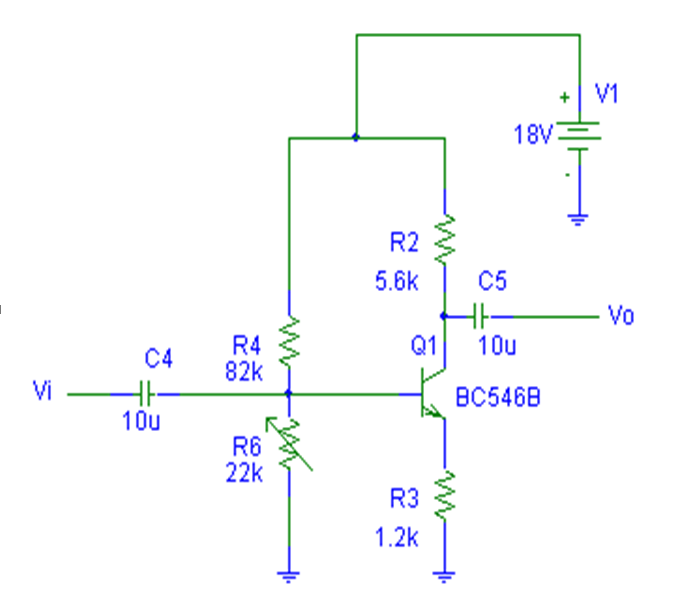
\includegraphics{Media/transistor_circuit.png}
        \caption{Transistorkrets for beregninger}
        \label{fig:circuit}
    \end{figure}

    \subsection{Undersøke egenskaper ved spenningsdeler krets}
        Hensikten med denne deloppgaven er å undersøke hvordan endringer i verdier for $I_C$ påvirker $V_C$, $V_E$ og $V_{CE}$. I tillegg undersøke hva som skjer med $I_C$ når spenningen $V_{BE}$ endres.

        \subsubsection{$I_C$ når $V_{BE}$ endres}
            Ser man på input karakteristikken vist i figur \ref{fig:common_emitter_characteristics}
            \begin{figure}[H]
                \centering
                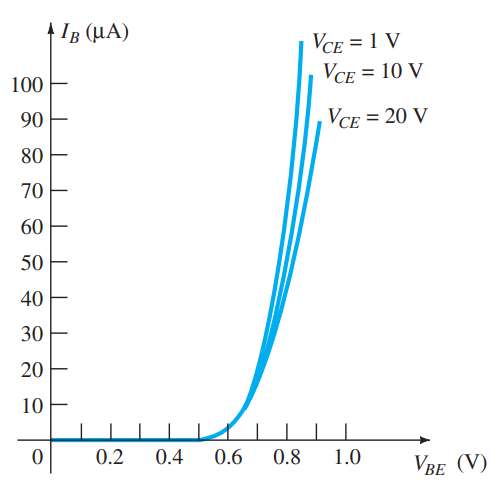
\includegraphics{Media/commonemitter_characteristics.png}
                \caption{Felles-emitter karakteristikk}
                \label{fig:common_emitter_characteristics}
            \end{figure}            
